\documentclass[letterpaper, 12pt]{article}

\usepackage{graphicx}
\usepackage{longtable}
\usepackage{rotating}
\usepackage{dcolumn}
\usepackage{listings}
\usepackage{subfiles}
\usepackage{amsmath}
\usepackage[margin=0.5in]{geometry} % for more room on the pages :)

% Code listing commands
\lstset{language=R,
basicstyle=\scriptsize\ttfamily,
commentstyle=\ttfamily,
numbers=left,
numberstyle=\footnotesize,
stepnumber=1,
numbersep=5pt,
showspaces=false,
showstringspaces=false,
showtabs=false,
frame=single,
tabsize=2,
captionpos=b,
breaklines=true,
breakatwhitespace=false,
title=\lstname,
escapeinside={},
keywordstyle={},
morekeywords={}
}

\renewcommand\thesection{Part \Alph{section}:}
\renewcommand\thesubsection{(\roman{subsection})}
\newcommand{\ind}[1]{\textbf{1}\{#1\}}

\graphicspath{{img/}}

\begin{document}
\title{ARE213 Problem Set \#3}
\author{Peter Alstone \& Frank Proulx}
\maketitle

\section{Linear models to motivate RD}

\subsection{LM results comparison}

\subfile{tab1a.tex}

Using a series of linear models (with heteroskedasticity consistent ``robust" standard errors), we find that for a range of model formulations there is a significant effect on housing price from the presence of hazardous waste cleanup sites, but not in the direction one would expect.  Instead of a reduction in housing value we estimate an increase in the value, which does not seem likely to be true.  The coefficient for the hazardous waste indicator variable (npl2000) takes a wide range of values depending on which additional explanatory variables are included in the model, from 0.04 (i.e., approximately a 4\% increase) for the simple model only including 1980 housing values and npl2000 to estimate 2000 housing values, to 0.09 for a model including both housing and demographic characteristics.  

\paragraph{Requirements for Unbiased Estimates [add to this]:}For our estimates to be unbiased we would need to include all of the potential sources of variation in housing price in a linear model.  A particular challenge is that there are very few sites with NPL2000 status (only 2\% of sites), so while the overall sample size is large there is very little support for estimates related to NPL2000 status compared to other covariates.  Critically, the overlap assumption must hold for the regression to be successful.  

\subsection{Comparing covariates}

We compare the covariates between census tracts and sites in a series of contingency tables and find that there are wide disparities between census tracts with and without NPL2000 status.  This erodes confidence that there is support in the data to use tract-level linear regression models, since the overlap assumption may be violated from wide differences in the other characteristics on the tract level.  On the site level, simply comparing over / under the trigger limit for the national priorities list (HRS score of 28.5) seems to solve some but not all the problems with overlap.  While many covariates cannot be said to come from different distributions there are still some that have significant differences.  Narrowing into a window from 16.5 - 40.5 (with the 28.5 dividing line) results in comparisons for which the hypothesis that the covariates are from the same distribution is not rejected.  Overall, these comparisons motivate the regression discontinuity design.  By narrowing in on a region where overlap in distribution for the covariates holds we have a fighting chance to identify a treatment effect, albeit with difficulty in establishing external validity.  

\subfile{tab1b-1.tex}
\subfile{tab1b-2.tex}
\subfile{tab1b-3.tex}

\section{RDD setup}
Based on the plot of the density distribution (Figure \ref{fig:ddplot}) using default values for bandwidth and bin width ($h \approx 12.6$, $b \approx 1.6$), it does not appear that there is a significant discontinuity in the neighborhood of HRS=28.5. The estimated value lines appear to nearly match with each other, and more importantly the upperbound 95\% C.I. for values below HRS=28.5 and the estimated value above HRS=28.5 overlap, and vice versa for the lowerbound 95\% C.I. for values above HRS = 28.5. This has us convinced that the Regression Discontinuity Design is not appropriate around this value. In addition, this lack of discontinuity appears to be consistent across various bandwidth values (tested with values $h = \{4, 8, 16, 20\}$).

\begin{figure}[htbp]
\begin{center}
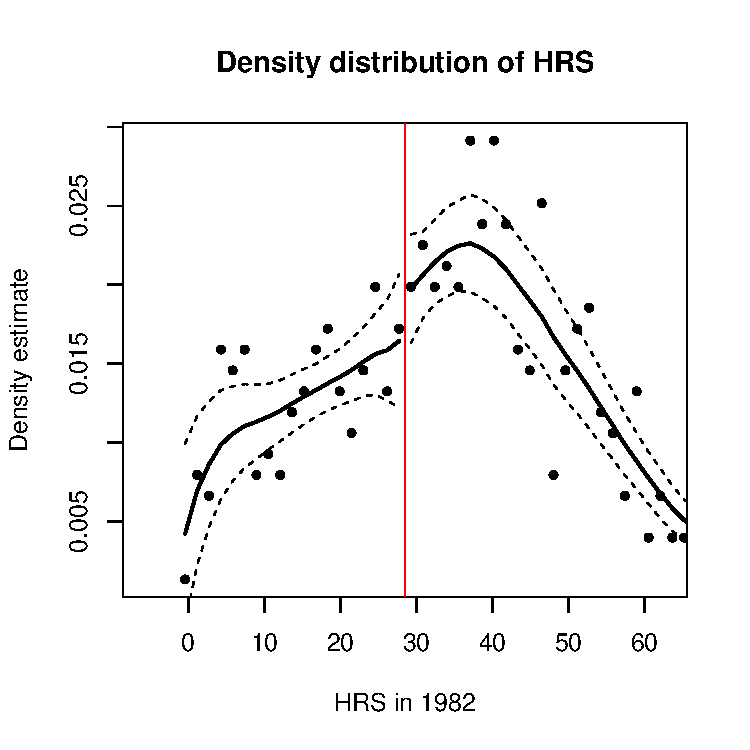
\includegraphics{ddplot.pdf}
\caption{Density distribution histogram for 1982 HRS.}
\label{fig:ddplot}
\end{center}
\end{figure}

NOTES: The way they picked is good, it means that 28.5 is not some magic number above which things get demonstrably worse but is as good as random.  So any discontinuity is due to the vagaries of program design and not endogenous variation.

\section{RDD First Stage}
The first stage equation is $\ind{NPL_{2000}}=\gamma_1HRS_{82}+x_i\gamma_2+u_i$.

\section{RDD Second Stage}

\section{Synthesis}

\section{Appendix: Code Listings}

\lstinputlisting{../util/are213-func.R}

\end{document}
